\begin{figure}
	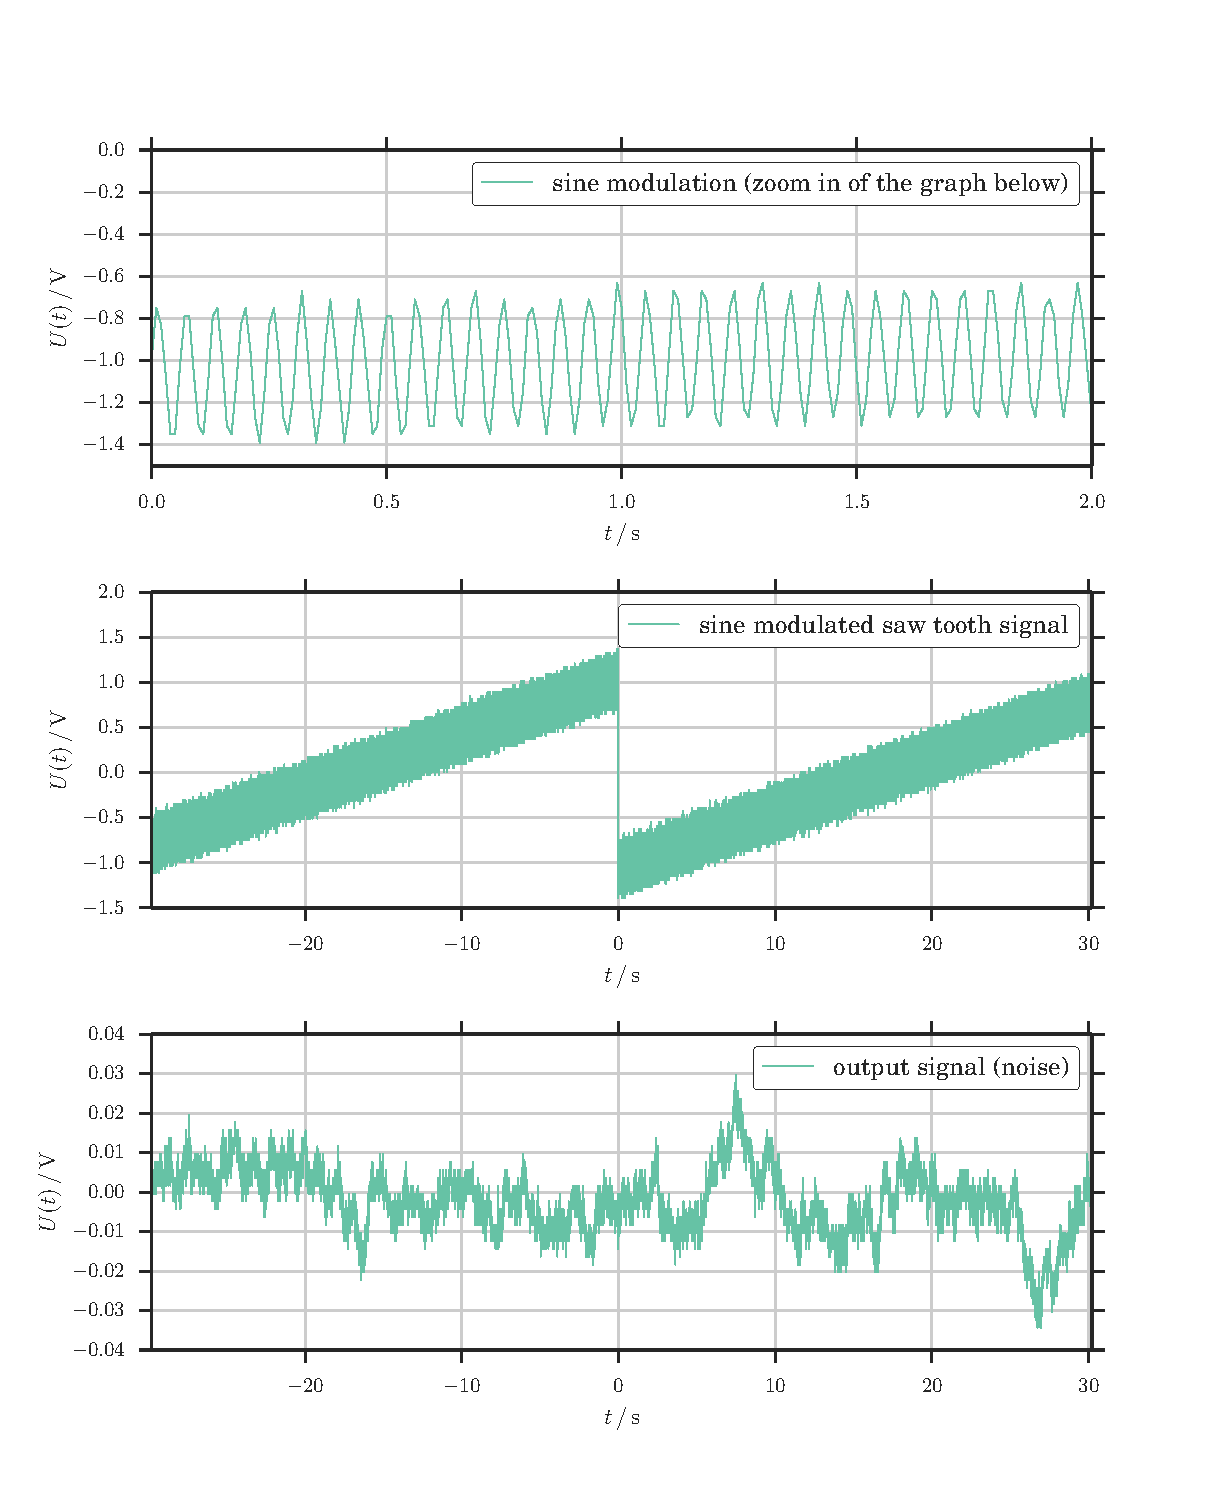
\includegraphics[width=\textwidth]{figures/example.pdf}
	\caption{
		Example for failure of the lock-in method.
		The upper two graphs show the sine modulated saw tooth signal
		in two different ranges for $t$. The zoomed range of the uppermost 
		graph can be used to calculate the frequency of the sine modulation.
		The output signal is basically noise, no absorption signal can be observed.
		}
	\label{fig:lock_in_example}
\end{figure}

